%%%%%%%%%%%%%%%%%%%%%%% file template.tex %%%%%%%%%%%%%%%%%%%%%%%%%
%
% This is a general template file for the LaTeX package SVJour3
% for Springer journals.          Springer Heidelberg 2010/09/16
%
% Copy it to a new file with a new name and use it as the basis
% for your article. Delete % signs as needed.
%
% This template includes a few options for different layouts and
% content for various journals. Please consult a previous issue of
% your journal as needed.
%
%%%%%%%%%%%%%%%%%%%%%%%%%%%%%%%%%%%%%%%%%%%%%%%%%%%%%%%%%%%%%%%%%%%
%
% First comes an example EPS file -- just ignore it and
% proceed on the \documentclass line
% your LaTeX will extract the file if required
%\begin{filecontents*}{example.eps}
%%!PS-Adobe-3.0 EPSF-3.0
%%%BoundingBox: 19 19 221 221
%%%CreationDate: Mon Sep 29 1997
%%%Creator: programmed by hand (JK)
%%%EndComments
%gsave
%newpath
%  20 20 moveto
%  20 220 lineto
%  220 220 lineto
%  220 20 lineto
%closepath
%2 setlinewidth
%gsave
%  .4 setgray fill
%grestore
%stroke
%grestore
%\end{filecontents*}
%
\RequirePackage{fix-cm}
%
%\documentclass{svjour3}                     % onecolumn (standard format)
%\documentclass[smallcondensed]{svjour3}     % onecolumn (ditto)
%\documentclass[smallextended]{svjour3}       % onecolumn (second format)
\documentclass[twocolumn]{svjour3}          % twocolumn
%
\smartqed  % flush right qed marks, e.g. at end of proof
%
\usepackage{graphicx}
\usepackage{slashbox}     
\usepackage{subfigure}
\usepackage{breakcites}

%
% \usepackage{mathptmx}      % use Times fonts if available on your TeX system
%
% insert here the call for the packages your document requires
%\usepackage{latexsym}
% etc.
%
% please place your own definitions here and don't use \def but
% \newcommand{}{}
%
% Insert the name of "your journal" with
% \journalname{myjournal}
%
\begin{document}

\title{Identifying Values to Express Emotions with a Non-Anthropomorphic Platform%\thanks{Grants or other notes
%about the article that should go on the front page should be
%placed here. General acknowledgments should be placed at the end of the article.}
}
%\subtitle{Do you have a subtitle?\\ If so, write it here}

%\titlerunning{Short form of title}        % if too long for running head

\author{Julian M. Angel-Fernandez         \and
        Andrea Bonarini %etc.
}

%\authorrunning{Short form of author list} % if too long for running head

\institute{Julian M. Angel-Fernandez \at
              Automation and Control Institute, Vienna University of Technology,\\ Karlsplatz 13, 1040 Vienna, Austria \\
              Tel.: +43-158801\\
              \email{jangelfe@tuwien.ac.at}           %  \\
%             \emph{Present address:} of F. Author  %  if needed
           \and
           Andrea Bonarini \at
              Andrea Bonarini, Dipartimento di Elettronica, Informazione e Bioingegneria,Politecnico di Milano,\\
              Piazza Leonardo da Vinci 32, 20133 Milan, Italy \\
              \email{andrea.bonarini@polimi.it}
}

\date{Received: date / Accepted: date}
% The correct dates will be entered by the editor


\maketitle

\begin{abstract}
Although anthropomorphic embodiment may support robot acceptance in interactive tasks, there are robots that cannot have a humanoid shape, and still have to interact with humans. As a consequence,  features not related with shape should be exploited to support robot acceptance. This paper presents an experiment made to understand the contribution to humans' perception of emotion of angular and linear velocity, body orientation, and movement direction of a non-anthropomorphic robot. A top 10 table of feature values combination was created for each enlisted emotion using alpha agreement for the whole treatment and for the desired emotion. The obtained results suggest values that could guide the implementation of the considered emotions in social robots.
\keywords{Robot-Human Interaction \and Emotion Projection}
% \PACS{PACS code1 \and PACS code2 \and more}
% \subclass{MSC code1 \and MSC code2 \and more}
\end{abstract}

\section{Introduction}
The development of fast, cheap, and reliable electronics has enabled the creation of new devices and versatile robotic platforms. These new platforms' capabilities have expanded the frontiers of the robots applications  to new environments where robot are expected to interact with humans, such as health care, and house cleaning, among others. However, bringing robots in these environment raises the challenge to increase robots' acceptance. Although this could be seen as an easy task that just would need improvements in robots' appearances and capabilities, it is possible that people would expect to treat robots as humans has  as they do with computers.~\cite{Reeves1996}, which makes necessary the creation of robots that fulfil this expectations.

Some researchers have suggested that embedding emotion expression capabilities to robots could improve their acceptance in social environments~\cite{Pavia2014}. As consequence researchers~\cite{Breazeal2002,Arras2012} have added specific emotional poses and expression to their robots. Others have studied how to convey emotions with specific platforms~\cite{Li2011,Brown2014}. Nevertheless, these works have created modules to show emotions that are strongly integrated to their solutions, which eliminate the possibility to re-use or adapt their systems into other projects.

In theory, the projection of emotion with humanoid embodiments could be simplified to mimic the same movements that humans. However, this idea is not possible due robots physical limitations. Therefore, an exact matching of humans’ movements to convey emotions could not be used in robots \cite{Saerbeck2007,Canamero2010}. Therefore diverse researchers are studying diverse features and values to express emotions with different platforms. As a consequence, these results could not be widely used due to the differences of the platforms.

This paper presents an Emotional Enrichment System (EES), which modify actions' parameters and add additional actions to create the illusion of emotion expression in a robot. Although the EES was originally conceived to be used in an autonomous performance robot~\cite{angel2013} to enrich actions with emotions, its design was devised to make it extendable to other platforms and adaptable to new tasks. To achieve this goal, the system relies on an Emotional Execution Tree (EXT), which is based on simple actions, sequential and parallel nodes. Additionally, it is used the concept of compound actions to group a bunch of nodes, which reduces the tree dimension and allows the reuse of recurrent actions  generated by specific combinations of simple actions and other nodes. This EXT has been formalized to give a guideline to further implementations and extensions.
 
The rest of the paper is organized as follows. Section~\ref{sec:related_work} provides a brief overview of particularly relevant work related to our system. Section~\ref{ref:theatre} gives a brief explanation on TheatreBot architecture. Section~\ref{ref:general_system} gives a general introduction to the system ideas. Section~\ref{sec:emotional_execution_tree} gives the basic formalization of our system and principal components terms used on it. Section~\ref{sec:implementation} describes the implementation of the system and shows two demonstrations done with the system using platforms with different capabilities.
\section{Related Work}

It is not possible to apply a direct mapping from human studies to robots~\cite{Saerbeck2007,Canamero2010}. Nevertheless works done in human studies provide guidelines about possible features and values that could be used to generate emotional motion. 

\subsection{Human Studies}

Emotion plays an important role in human-human interaction and can be expressed through diverse channels such as body gestures and poses, body movements, face expressions. The human face is a complex structure that embraces more than 43 muscles act. Hence, the face has been considered as a primary channel to express emotion. As a consequence, many works have focused on facial expression, mainly but not only, influenced by the work done by Ekman~\cite{Ekman2004}. However, the role that body plays in emotion projection has been recognized and it has been started to be studied~\cite{Gelder2008,Wallboot1998}. Nevertheless, the amount of works related to body expression of emotions is still small compared to studies about facial expression. 

Analysing some of the few works that have studied human body expressiveness, it is possible to recognize two different methodologies to create the data base of movements to be assessed during the experiments. The first methodology uses human actors (either professionals or amateurs) to walk straight from point A to point B conveying specific emotions~\cite{Dael2012,Meijer1989,Wallboot1998}. Each trial is recorded and later shown to each subjects that have to classify all the sequences. The second methodology uses virtual agents~\cite{Roether2009,Venture2014} to generate the very same set up for the experiments; the agent's movements are generated from the data recorded from human actors.

The work done by Wallboot~\cite{Wallboot1998} has been used as a reference by other researches. It addressed the question: \textit{Are specific body postures indicative of emotion or are they only used to indicate the intensity of the emotion?} To answer this question, he recorded 224 videos for joy, happiness, sadness, despair, fear, terror, coldness anger, hot anger, disgust, contempt, shame, guilt, pride, and boredom, and showed them to the subjects. His results reaffirm that movement and body postures are indicative of intensity for some emotions. But at the same time, these two characteristics seem to be enough to identify other emotions. 

Complementary studies using virtual agents have been performed by  Kluwer and collaborators~\cite{Kluwer2004}, who studied the contribution of postures and angle view in the interpretation of emotions. They generated 176 static positions for happiness, anger, disgust, fear, sadness and surprise. Each image was later rendered from three different angles (front, left, and above and behind left shoulder) producing a total of 528 images. All the participants were exposed to all 528 images and were asked to label the image with the emotions that best represent it. Their results show that five out of six emotions were quite well recognized independently from the angle of view., while disgust was for some postures confused with fear.

There are two main drawbacks of all these projects that use video recorded sequences. First, they miss the impact related to a complete physical experience. For instance, it is clearly different facing an angry robot really rushing against us, or looking at a video where this happens. Second, each actor has his/her own way to represent a given emotion~\cite{Russell2003,Gunes2011}. Actors use diverse techniques to create believable representations of specific emotions. However, this does not ensure that all actor convey emotions in same way. Therefore, several records are done and the ones with the highest agreement are selected. This brings the technical question on how to interpret the significance of agreement obtained~\cite{Russell2003}.

\subsection{Robotic Studies}
%%%%%%%%%%%%%%%%%%%%%%
As a direct consequence of the abundance of works in face elicitation in humans, most of the works done in Human-Robot Interaction (HRI) have focused also on faces. One of the most well-known expressive robots is Kismet~\cite{Breazeal2002}, a robotic face able to interact with people and to show emotions. The face had enough degrees of freedom to portray the basic emotions suggested by Ekman~\cite{Ekman2004} (happiness, surprise, anger, disgust, fear, and sadness), plus interest. 
Despite the complex system behind Kismet, the emotion's projection evaluation was done using videos with a very limited number of participants. Similar approach was followed by Li and Chignell~\cite{Li2011}, who used videos of a teddy bear robot to study the contribution of arms and head movement to express emotions. In same direction Destephe and collaborators~\cite{Destephe2013b,Destephe2013} studied the attribution of emotion to a robot's gait using a virtual representation of the platform WABIAN-2R. More recently Knight and Simmons~\cite{knight2016} used Keepon and NAO platforms to study the possibility to project inner states with just head movements. Although use of videos has the advantage to cover a major number of participants, the lack of interaction with the real platform make these works lose the impact that a robot could generate on the participants.  

%%%%%%%%%%%%%%%%%%%%%%%%
The use of real platforms to study emotion projection could be dived in two lines: using anthropomorphic and non-anthropomorphic platforms. In the first case, these works are characterized by the use of cue positions to project desire emotions~\cite{NAO2013}. In some cases, special attention has been taken to determine head's angle and arms position contribution in specific emotions~\cite{Brown2014}. 
Nevertheless, current humanoid platforms cannot generate smooth gaits, which limit the study of body movements. For example Karg et al.~\cite{Karg2010} tried to map actors gaits on an hexadop robot to understand the contribution of step length, height and velocity. Their results suggest that using this approach is not suitable because the difference between different gaits are not recognizable. So they suggest that movements must be exagereted.  Some researchers have reduced the human appearance (e.g. eliminating limps and facial expressions)to increase platform mobility and study new mechanisms to project emotions~\cite{Arras2012}. Pushing forward the reduction on anthropomorphic features, Saerbeck and Christoph used a Roomba platform to study the contribution of curvature in a trajectory to conceive emotional states~\cite{Saerbeck2010}. Similarly Lourens and Barakova~\cite{BarakovaL10} implemented a set of behaviors to determine the emotion  perceived from diverse movements, which were selected from the  work done by Camurri et al.~\cite{pop00002}. Continuing with her research on how robotics' behaviours are interpreted by people, Barakova and collaborators~\cite{Barakova2013} created a closet in which lights could be manipulated to convey pre-defined behaviours. The robot's behaviours were defined using the Interpersonal Behaviour Circle (ICB)~\cite{Leary57}, which is based on two dimensions (dominance-submission and hate-love). Their findings suggest that electronic systems can elicit a type of reactions different from the one expected by theories of interpersonal communication.

Other approaches have tried to get a better understanding of the contribution of diverse features to express emotions through movement. For example, Suk and collaborators payed a particular attention to speed, smoothness, granularity of movement path and volume of a non-bioinspired object~\cite{NAM2014}. They used the self-assessment (SAM)~\cite{Lang2008} method to evaluate participants. Their results suggest that arousal increases as speed increases and that there is not any clear tendency for smoothness. On the other hand, granularity is positively correlated with pleasure and arousal, while volume is negatively correlated with pleasure and positively correlated with arousal. Alike, Tan and collaborators~\cite{Tan2016} have studied the contribution of velocity, fluidity, direction and orientation of a small box. They evaluated participants' perception using SAM. Their results suggest that direction is directly correlated with dominance, but that fluidity does not influence the perception. While flat orientation is related to positive valence, leaning position are related with negative valance. Finally the velocity is correlated with valence, arousal and dominance. Using an hexapod robot, Karg et al. studied 

Due to the popularity that quadrocoptors have received in the last years, Sharma and collaborators~\cite{Sharma2013} used a quadrotor to study how different Laban's effort~\cite{Laban1968} parameters could impact on the perception of affection. A professional Laban certified actor was asked to generate 16 different paths, for each one changing one of the four Laban's parameters (space, weight, time, and flow). Each generated path was recorded using the Vicon motion-tracking system. Continuing with the use of quadrocoptors, Cauchard and collaborators~\cite{Cauchard2016} studied how flight paths could project personal traits and emotional attributes. All these works present a very nice starting to point to identify features and values that could be used to project emotions in robotics, which could help in coordinating humans and robots~\cite{Novika2015}. However, all of these works not give a price guideline to elicit precise emotions, which from our previous case studies could lead to the misinterpretation of movements emotions~\cite{Angel2016}. For example people could confuse an implementation of \textit{Happiness} with \textit{Anger}.
\section{The System}
\label{sec:system}

The system used in the experiment is composed by a non-anthropomorphic platform and software architecture that enrich robot's movements with emotion. The robotic platform was envisioned to be as simpler as possible to let the study of the desired characteristics. 

%%%%%%%%%%%%%%%%%%%%%%%
\subsection{Hardware and Mechanical}

A holonomic platform was built to be used in the experiment. This type of platforms are characterized by the possibility to move in any direction without the necessity to have a specific orientation, i.e., they are free to move taking any desired orientation. Therefore, it was possible to imitate movements that are done by humans. For example, people move straight even if they turn their whole body a bit. The platform has a diameter of 25 cm and height of 25 cm. Figure~\ref{fig:ThirdDesign} shows the platform's blue prints and the real platform. Robot's frame of reference, in which all the velocities are going to be calculated, are depicted by the two black arrows. So, as it could be observed, to make the robot move forward it must be send a velocity in $y$ axis.

\begin{figure}
	\centering
	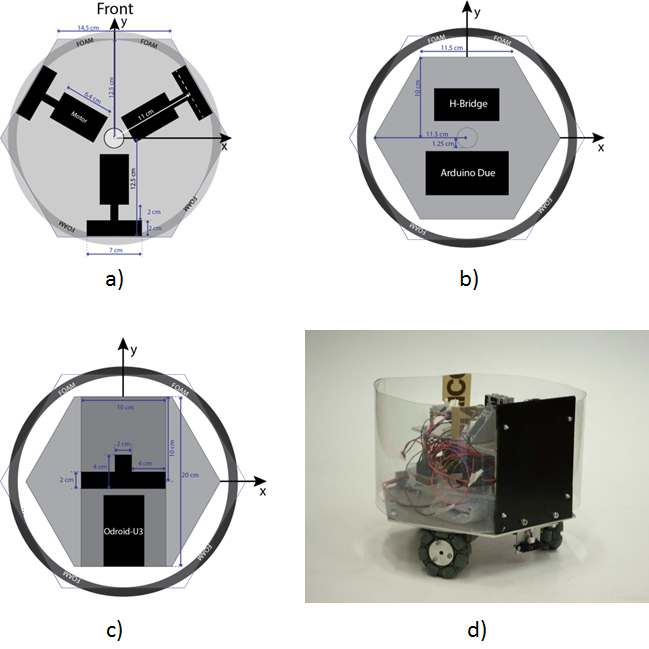
\includegraphics[width=0.8\textwidth]{Images/DesignThird.png} 
	\caption{Design of the platform. a) Base platform, this layer is used to carry the batteries. The two black arrows represent robot's frame of reference. b) First layer, which includes the Arduino and the H-Bridges to control the motors. c) Second layer with the Odroid-U3 and the mechanical structure to support the upper part. d) Lateral view of the version.}
	\label{fig:ThirdDesign}
\end{figure}

%%%%%%%%%%%%%%%%%%%%%%%platform_base
\subsection{Software}
To ensure robot's velocity it was implemented a PID controller for each motor. PID's set point is established by a controller that could receive two different types of commands. The first commands is robot's velocities ($<V_x,V_y,\omega>$), which are given in robot's frame of reference. The second command is a point ($<x, Y, \theta>$), which is given in the general frame of reference. This frame of reference is set every time the system is reset or boot. For example, if the robot finishes a trajectory and then it is reset, the new frame is going to be in the robot's current position.  

Additional to this low level control, it was created a graphical interface~\ref{fig:experimental_interface} to reduce the possibility on introducing wrong values for a desired sequence. This interface loads the sequences from a .txt file and displays sequences' numbers on it. Every time that a new sequence should be presented to a participant, the sequence's number is selected in the interface, which will display sequence's values. Once the robot has been positioned to the correct position, the execution could be started by clicking on send button. Here two commands are send, one resetting the controller and the second the desire position. In case that the sequence's execution should be aborted, it should be clicked the button stop.

\begin{figure}
	\centering
	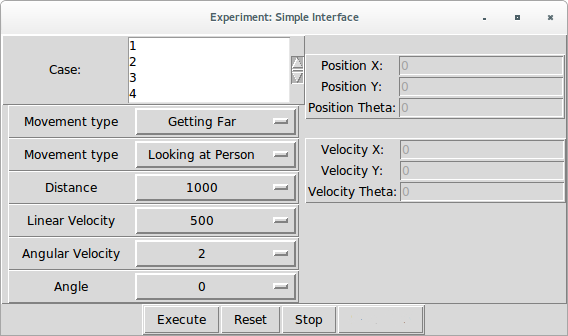
\includegraphics[width=0.60\textwidth]{./Images/ExperimentInterface.png} 
	\caption{Interface used in the experiment. Once a sequence is selected, the interface shows sequence's values. Also, the interface give information about the current position of the robot and its velocity.}
	\label{fig:experimental_interface}
\end{figure}
\section{Experimental Design}
\label{sec:experiment}

The experiment was designed to get a better understanding about the contribution linear and angular velocity, oscillation angle, direction, and orientation to express happiness, anger, sadness and fear, which are four out of six emotions considered by Ekman~\cite{Ekman2004} as basic emotions.
%%%%%%%%%%%%%%%%%%%
%%%%%%%%%%%%%%%%%%%

\subsection{Independent Variables}

The definitions of the selected independent variables are reported here below.

\begin{itemize}
	\item \textbf{Angular velocity} is the rotational speed  ($\omega$) of the robot with respect to its center.

	\item \textbf{Oscillation angle} is the maximum extension in which the robot will rotate around its center in the oscillating movement ($\theta$).

	\item \textbf{Linear velocity} is the rate of change of the position of the robot ($V$). 

	\item \textbf{Direction with respect to participant's perspective} is the angle generated from the participant's point of view with respect to the robots trajectory ($D$).

	\item \textbf{Orientation of the body with respect to participant's perspective} is the robot's body orientation with respect to the robot's trajectory ($\phi$).

\end{itemize}

The three first variables are shown in Figure~\ref{fig:angular_movement}. As it could be observed, robot's frame of reference is draw to show that it could move straight while is rotating.


\begin{figure}
	\centering
	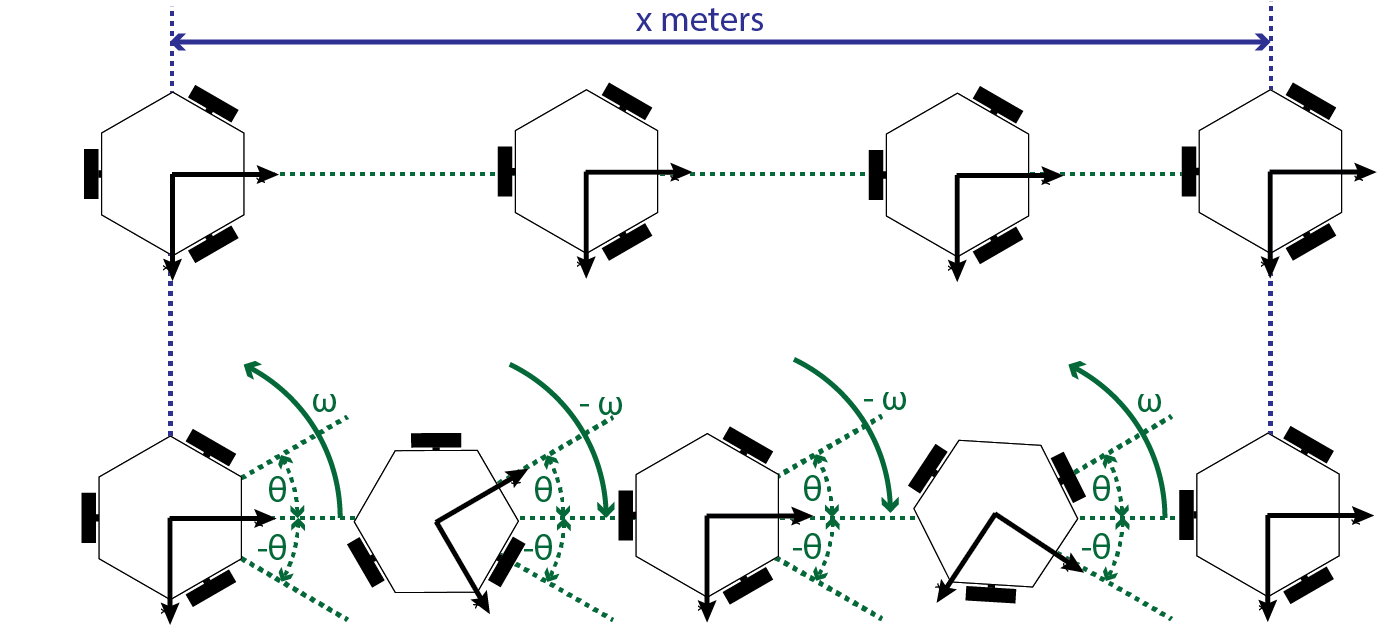
\includegraphics[width=0.80\textwidth]{./Images/ExampleMovement.png} 
	\caption{Example of the features used in the experiment. $x$ represents the displacement in meters, $\omega$ is the angular velocity ($rad/s$) and $\theta$ the oscillation of the body around its center ($rad$). The upper sequence depicts a movement based only on linear velocity, while the bottom one shows a sequence with angular and linear movement. The two black arrows in the robot's middle depict robot's frame of reference.}
	\label{fig:angular_movement}
	
\end{figure} 

%%%%%%%%%%%%%%%%%%%
%%%%%%%%%%%%%%%%%%%
\subsection{Dependent Variables}

\begin{itemize}
	\item \textbf{Emotion:} is the feeling perceived by the participants from the robot's movement. From previous experiences %TODO cite
	, it was decided to ask the participants to select an emotion name in a list including the four emotions intended to be expressed,  two mental states that could be misinterpreted from these emotions, and the option of ``other'', where participants could write their own interpretation. 
	The two  states of mind included as confounding terms are tenderness and excitement, which correspond to low and high arousal states.
	
	\item \textbf{Emotion's intensity:} indicate the emotion intensity as perceived by the subject. This variable is measured on a ten point scale rate, ranging from 0 to 10, where 0 means that the corresponding emotion is not perceived by the subject and 10 that the emotion is highly perceived by the subject. 

\end{itemize}
%%%%%%%%%%%%%%%%%%%
%%%%%%%%%%%%%%%%%%%
\subsection{Independents' Variables Values}

It was decided to select specific for all independents variables, discrete values to make the experiment feasible. First, a simple test to evaluate when significant changes could be perceived was performed on a small sample of independent subjects. Base on this test specific values for oscillation angle, and angular and linear velocities were selected. For the remaining two variables were selected the cases that could be beneficial for the experiment. 
The chosen values are shown in Table~\ref{table:variables_values}. 

\begin{table}[htb]
\caption{Possible values for each of the independent variables.}
\begin{tabular}{|c|c|c|c|c|}
\hline
\backslashbox{Variable}{Possibilities} & First & Second & Third & Fourth\\
\hline   
Angular Velocity ($rad/sec$)& $0$ & $1$ & $2$ & $3$\\
\hline
Oscillation Angle ($rad$)& $0$ & $0.087$ & $0.175$ & $0.349$\\
\hline
Linear Velocity ($mm/sec$) & $0$ & $200$ & $500$ & $900$\\
\hline
Direction ($rad$)&$0$&$\pi$&$\frac{-\pi}{2}$& \\
\hline
Orientation ($rad$) & $0$ & $\pi$ & & \\
\hline 
\multicolumn{5}{c}{}
\end{tabular} 
\label{table:variables_values}
\end{table}

To get a better idea about the Direction and Orientation values, in Figure~\ref{fig:possibilities_orientation_direction} are reported all the possibilities for these two variables.

\begin{figure}
	\centering
	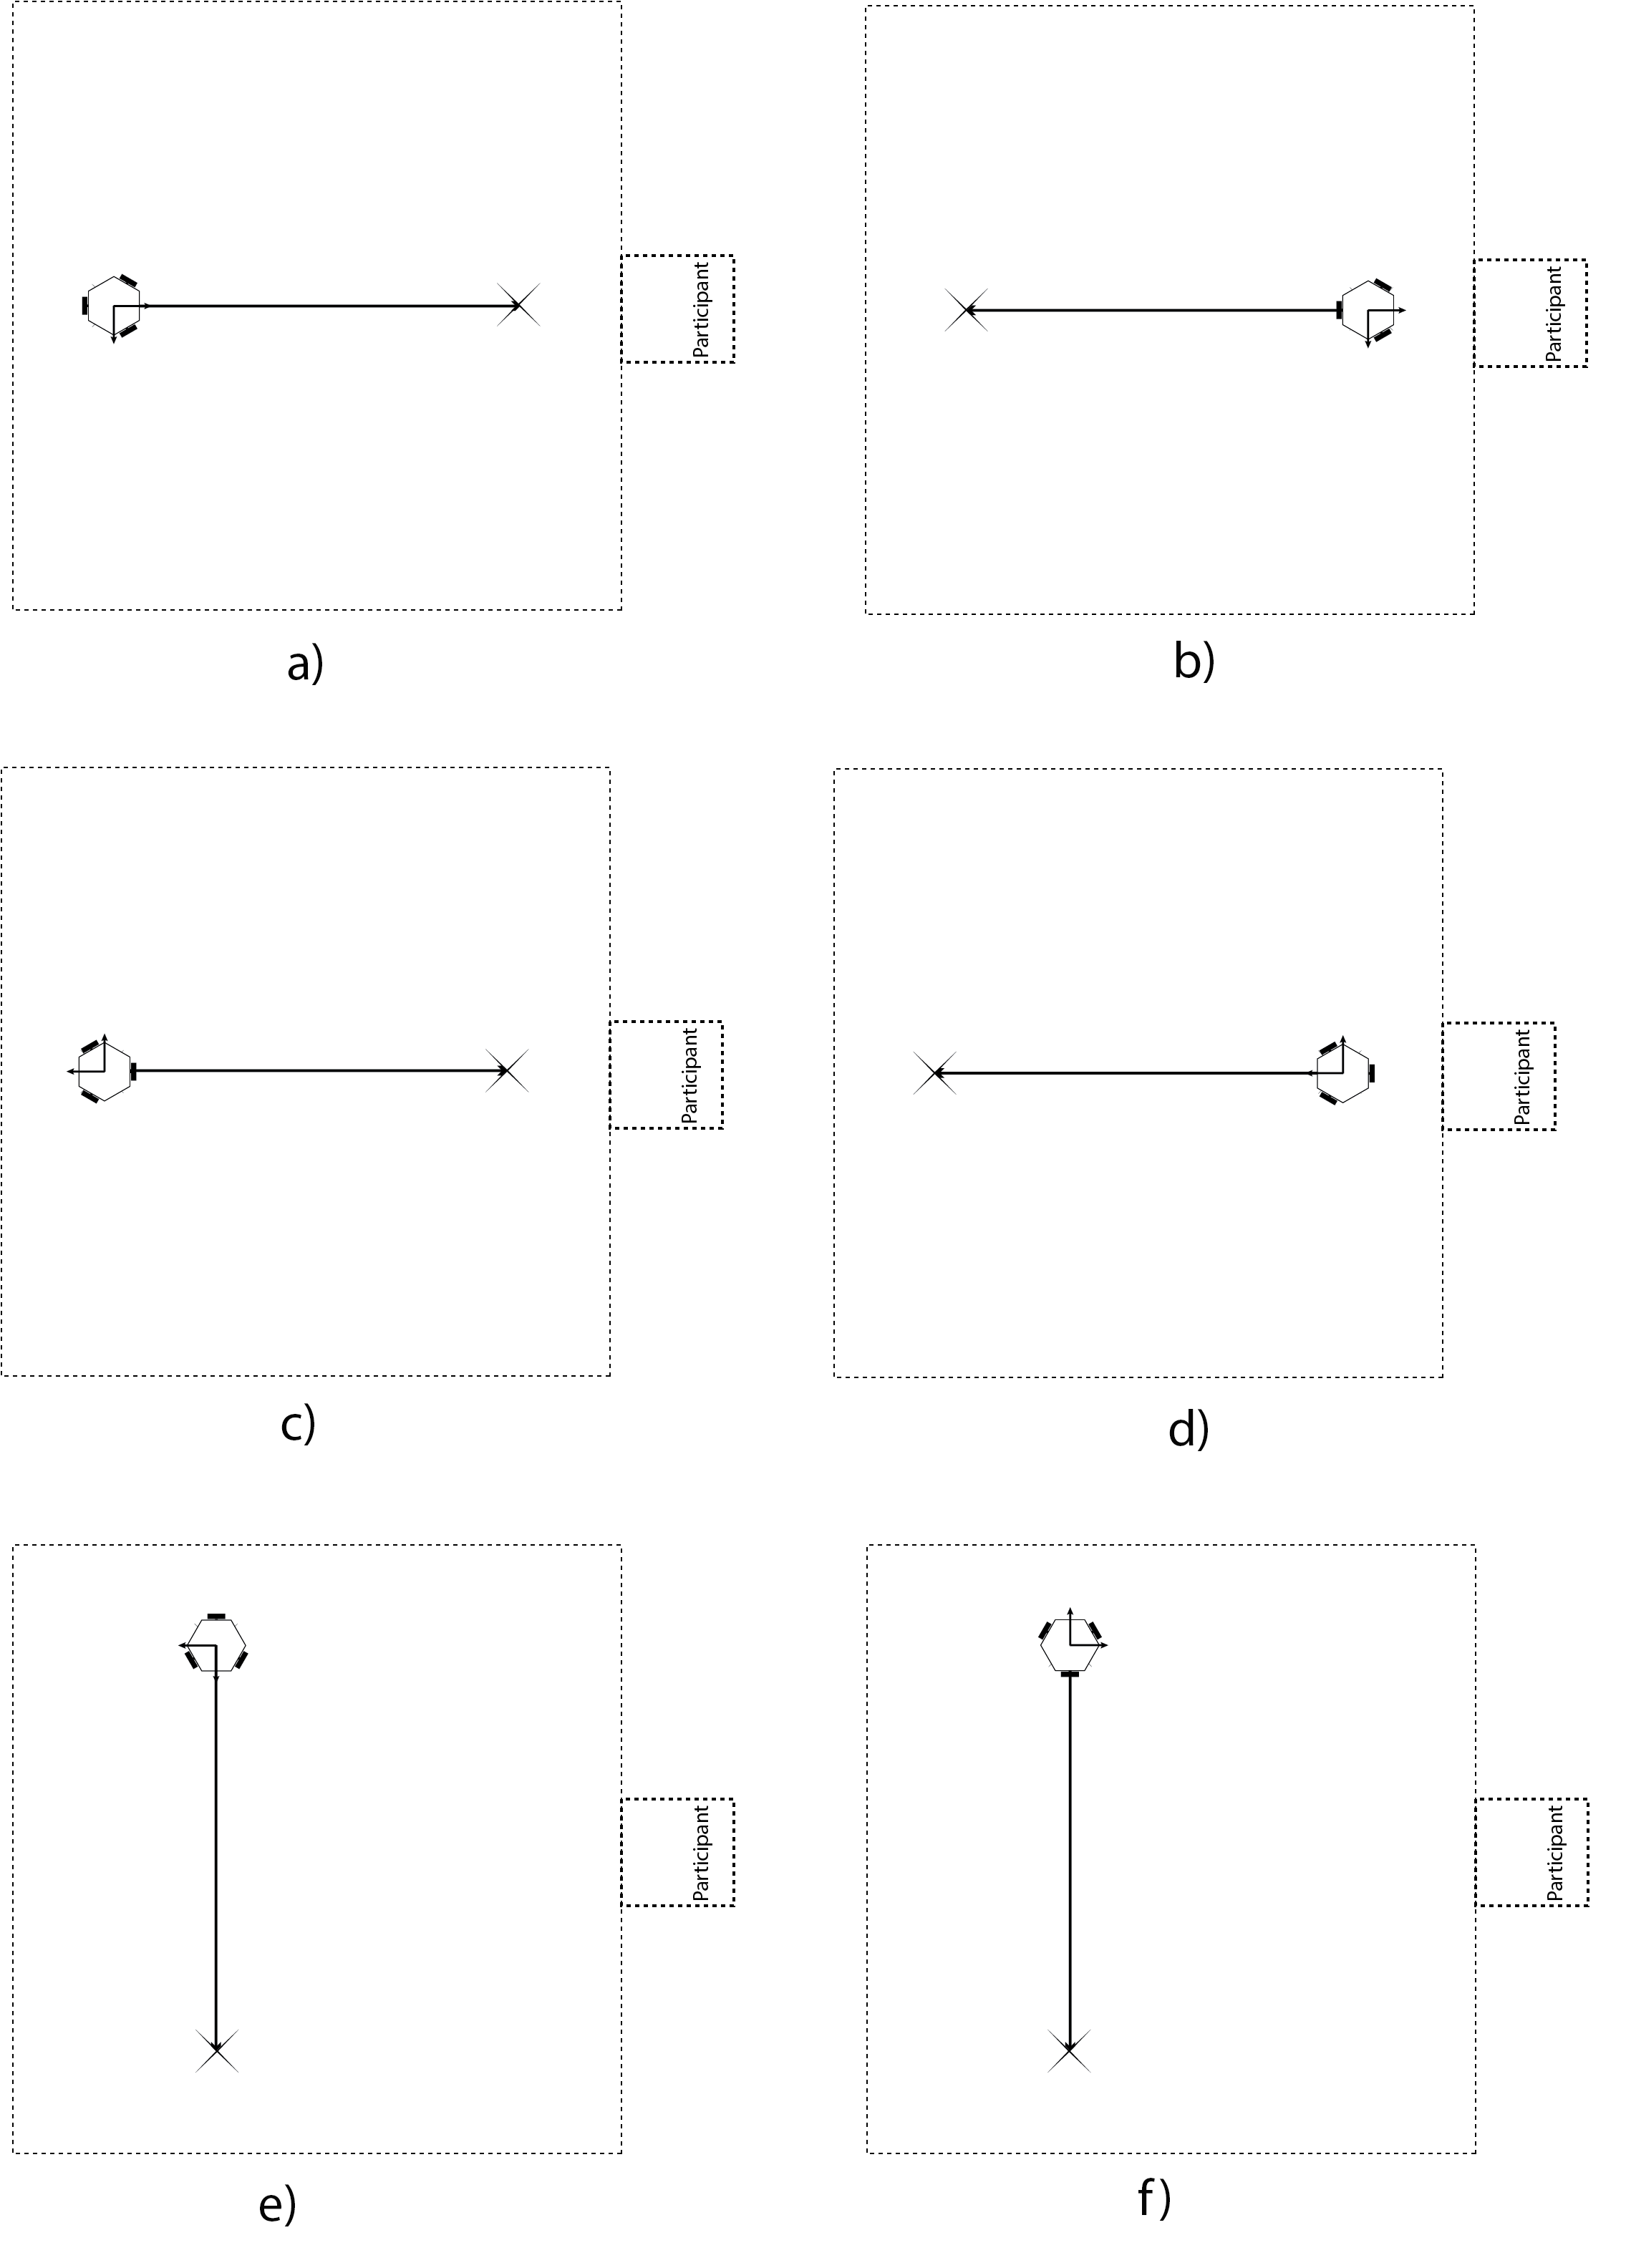
\includegraphics[width=1.0\textwidth]{./Images/possibilities_case.png} 
	\caption{Combination of direction and orientation. The crosses symbolize the final position. The robot represents the initial position with its orientation, which is represented through the robot's frame of reference. The dash big square represents robot's movement zone, while the small represents participant's zone. a) Direction = $0$ and Orientation = $0$. b) Direction = $0$ and Orientation = $\pi$. c) Direction = $\pi$ and Orientation = $\pi$. d) Direction = $\pi$ and Orientation = $0$. e) Direction = $\frac{-\pi}{2}$ and Orientation = $0$. f) Direction = $\frac{-\pi}{2}$ and Orientation = $\pi$}
	\label{fig:possibilities_orientation_direction}
\end{figure}

The experiences, meant as desired procedures to compare~\cite{oehlert2000first}, were generated from the combination of independent variables' values for a total of 384 combinations. All the experiences that would not add any significant information to the experiment were deleted, such as experiences with $\theta=0$ and $\omega \neq 0$, which reduced the total amount of treatments to 195.

%%%%%%%%%%%%%%%%%%%
%%%%%%%%%%%%%%%%%%%
\subsection{Participants' Sequence}

It was decided that each subject will be just exposed to twenty over one hundred and ninety five possible experiences, which lasted  from 10 to 15 minutes. This was decided because each subject was a volunteer and would not perceive any monetary remuneration, so the time dedicated to the experiment had to be kept limited. The twenty treatments were selected picking a number without replacement from 1 to 195.
%%%%%%%%%%%%%%%%%%%
%%%%%%%%%%%%%%%%%%%

\subsection{Setup}

The experiment's setup and dimensions are shown in the Figure~\ref{fig:setup}. The crosses symbolize possible starting points, which were selected depending on the direction's value, as it is showed in Figure~\ref{fig:possibilities_orientation_direction}. 

\begin{figure}
	\centering
	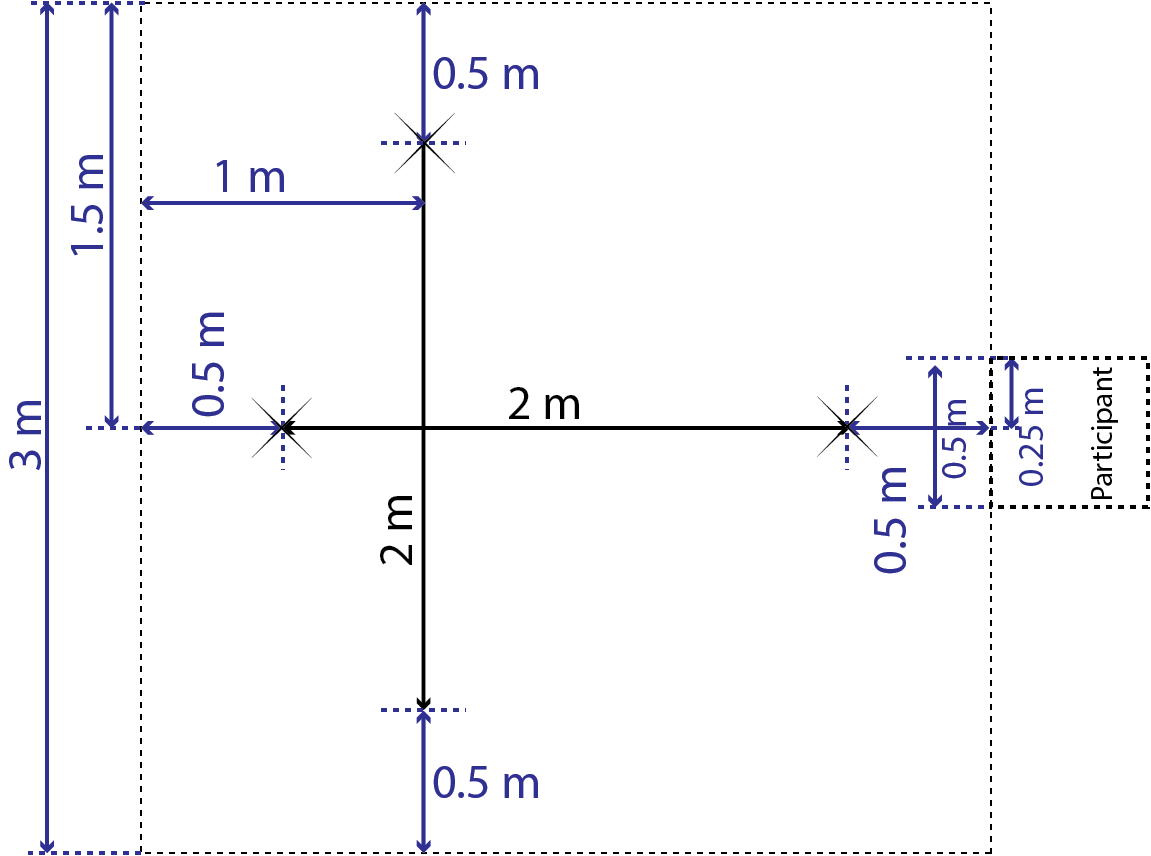
\includegraphics[width=0.50\textwidth]{./Images/ExperimentGeneral.png} 
	\caption{Setup for the experiment. The crosses symbolize the possible starting points.}
	\label{fig:setup}
\end{figure} 
\section{Results}
\label{sec:result}
This section reports the results obtained during two days for the two parts of the case study.

\subsection{Part I: Emotion Recognition}

The results obtained from the presentation of emotional movements are summarized in 
Table~\ref{table:result_fourth}. 
\begin{table}
\centering
\small
\caption{Summary of the answers obtained in the presentation of emotional movements.}
		\label{table:result_fourth}
		\begin{tabular}{|c|c|c|c|c|c|c|c|c|}
			\hline
\rotatebox{90}{\textbf{Presented/Reported } }&
\rotatebox{90}{\textbf{Happiness}}&
\rotatebox{90}{ \textbf{Anger}} &
\rotatebox{90}{\textbf{Fear}}&
\rotatebox{90}{\textbf{Sadness}}&
\rotatebox{90}{\textbf{Excitement}}&
\rotatebox{90}{\textbf{Tenderness}}&
\rotatebox{90}{\textbf{Other}}&
\rotatebox{90}{\textbf{Total}}\\	
			\hline
			Happiness-1&8&16&7&4&16&4&7&62\\
			\hline
			\co Happiness-2&\co 11&\co 11&\co 6&\co 2&\co 19&\co 3&\co 1&\co 53\\
			\hline
			Anger-1&7&5&6&2&21&7&1&49\\
			\hline
			\co Anger-2&\co 14&\co 29&\co 13&\co 2&\co 13&\co 3&\co 2&\co 76\\
			\hline
			Fear-1&6&2&28&1&9&6&0&52\\
			\hline
			\co Fear-2&\co 7&\co 3&\co 37&\co 2&\co 20&\co 4&\co 1&\co 74\\
			\hline
			Sadness-1&3&5&17&14&5&16&5&65\\
			\hline
			\co Sadness-2&\co 5&\co 5&\co 15&\co 28&\co 6&\co 15&\co 7&\co 81\\
			\hline
			\end{tabular}
\end{table}

It could be observed that both implementations of \textit{Happiness} were confused with \textit{Anger} and \textit{Excitement}. In a similar way, Anger-1 was mostly confused with \textit{Excitement}, which was voted twenty one over forty nine subjects.
Anger-2 shows an improvement of perception from 10\% to 38\%, respect Anger-1. This implementation was perceived also as \textit{Happiness}, \textit{Fear} and \textit{Excitement}.
Both implementations of \textit{Fear} had a high level of recognition 54 \% and 50 \% and mostly confused with \textit{Excitement}, which was voted nine times for the first implementation and twenty times for the second implementation. Finally, the two implementation of \textit{Sadness} were confused with \textit{Fear} and \textit{Tenderness}.

An analysis was done per groups, for each presented emotion. For each emotion it was considered how many subjects in each group recognized it, how many identified a different emotion, how many identified the considered emotion when presented another one, and how many subjects recognized an emotion different from the considered one when presented a different emotion. This lead to a table, which is known as contingency table, for each presented emotion, like the one reported in table~\ref{table:singleEmotion} for Happiness-1. 
\begin{table}[!htbp]
\begin{center}
\caption{Example of table compiled for each emotion on the subjects which have been presented each emotion (here Happiness-1).}
\label{table:singleEmotion}
\begin{tabular}{|c|c|c|}
\hline 
Presented/Reported&Happiness&Other\\
\hline 
Happiness-1&8&54\\
\hline 
Other&42&355\\
\hline
\end{tabular}
\end{center}
%\vspace{-0.5cm}
\end{table}

For each of the contingency table the classification accuracy and the no-information rate (NIR), i.e. the accuracy that had been obtained by random selection, are reported in Table~\ref{table:nir_fourth}. The results reveal that Sadness-2 is the only implementation that was correctly recognized among all implementations ($p<0.05$). 

\begin{table}
\centering
\small
		\caption{Classification accuracy of the presented emotions by the single panels, computed as mentioned in the text, with corresponding 95\% confidence interval, no-information rate, and p-value that accuracy is greater than the NIR.}		
		\label{table:nir_fourth}
			\begin{tabular}{|p{1.8 cm}|c|c|c|c|}
				\hline		
\rotatebox{90}{\textbf{Presented Emotion}}&
\rotatebox{90}{\textbf{Classification Accuracy}}&
\rotatebox{90}{\textbf{95\% CI}}&
\rotatebox{90}{\textbf{No-Information Rate}}&
\rotatebox{90}{\textbf{P-Value [Acc $>$ NIR]}}\\
				\hline
			Happiness-1&0.79&(0.75,0.82)&0.89&1.0\\
			\hline
			\co Happiness-2&\co 0.81&\co (0.77,0.84)&\co 0.88&\co 1.0\\
			\hline
			Anger-1&0.8&(0.76,0.83)&0.88&1.0\\
			\hline
			\co Anger-2&\co 0.89&\co (0.76,0.84)&\co 0.83&\co 0.95\\
			\hline
			Fear-1&0.79&(0.75,0.83)&0.88&1\\
			\hline
			\co Fear-2&\co 0.78&\co (0.73,0.81)&\co 0.83&\co 0.99\\
			\hline
			Sadness-1&0.85&(0.81,0.88)&0.84&0.47\\
			\hline
			\co Sadness-2&\co 0.85&\co (0.81,0.88)&\co 0.81&\co 0.035\\
			\hline
			\end{tabular}
\end{table}

Additionally, the positive predictive value, accuracy and a Pearson's $\chi^2$ were computed for each table. The hypothesis used in the test were:

\begin{itemize}
	\item $H_0 = $ there is a difference in recognition between the implementation respect the others.
	\item $H_1 = $ there is not a difference in recognition between one implementation respect the others.
\end{itemize} 

The results are shown in table~\ref{table:Precision2}. They show that there is significant evidence to conclude that Anger-2, both of \textit{Fear} and \textit{Sadness} are considered as a different implementation when they are compare with other implementations. While both implementations of \textit{Happiness} and Anger-1 are considered as similar to the other implementations. 

\begin{table}
\centering
\small
\caption{Accuracy, precision and results of Pearson's $\chi^2$ for each contingency matrix with $\alpha = 0.05$ for the case study.} 
\label{table:Precision2}
		\begin{tabular}{|p{1.6 cm}|p{1.5 cm}|c|c|c|}
		\hline
		\textbf{Presented Emotion} & \textbf{Positive Predicted Value} & \textbf{Accuracy} & \textbf{$\chi^2(1)$} & \textbf{p-value}\\
		\hline
		Happiness-1 & $0.13$ & $0.79$ & $0.11$ & $0.74$\\
		\hline
		\co Happiness-2 &\co $0.21$ &\co $0.81$ &\co $3.7$ &\co$0.054$\\
		\hline
		Anger-1 & $0.1$ & $0.8$ & $3.8e^{-29}$ & $1$\\
		\hline
		\co Anger-2 &\co $0.38$ &\co $0.81$ &\co $34.4$ &\co $<0.001$ 
		%4.47e-9
		\\
		\hline
		Fear-1 & $0.54$ & $0.8$ & $36.2$ & $<0.001$ 
		%1.8-e9
		\\
		\hline 
		\co Fear-2 &\co $0.5$ &\co $0.78$ &\co $35.8$ &\co $<0.001$ 
		%5.3e-10
		\\
		\hline
		Sadness-1 & $0.22$ & $0.85$ & $27.4$ & $<0.001$
		%$1.63e-7$
		\\
		\hline
		\co Sadness-2 &\co 0.35 &\co 0.85 &\co 72.9 &\co $<0.001$
		%2.2e-16
		\\		 
		\hline
			\end{tabular}
\end{table}  

To determine if which implementations were perceived as different or similar, a Fisher's exact test was applied for ten different combinations of the implementations. Additionally, a Holm-Bonferroni correction was applied for multiple comparisons to get a better p-value estimation. The following are the hypothesis used in this test:

\begin{itemize}
	\item $H_0 = $ there is a difference in the recognition of the two compared emotions.
	\item $H_1 = $ there is not a difference in the recognition of the two compared emotions.
\end{itemize}

The results are reported in Table~\ref{table:result_compare_fourth}. As it could be observed, both implementation of \textit{Anger} were perceived as two different emotions ($p<0.001$). Also shows that both implementation of \textit{Happiness} were perceived as to Anger-2 ($p=0.69$ in both cases).

\begin{table}
\centering
\small
\caption{Pair comparison among all the implemented emotions using Fisher's exact test for both questionnaires with $\alpha = 0.05$ for the  case study. The * indicates that the p-value was adjusted using the Holm-Bonferroni correction for multiple comparisons.}
		\label{table:result_compare_fourth}
		\begin{tabular}{|c|c|c|}
			\hline	
\textbf{Pair Compared} & \textbf{p-value} & \textbf{p-value*}\\	
			\hline
			Happiness-1 vs Happiness-2 &$0.38$&$1.0$\\
			\hline
			Anger-1 vs Anger-2 & $<0.001$ 
			%7.3e-4
			& $<0.001$
			%4.4e-3
			\\
			\hline
			Anger-2 vs Happiness-1 & $0.137$&$0.69$\\
			\hline
			Anger-2 vs Happiness-2 & $0.157$&$0.69$\\
			\hline
			Fear-1 vs Fear-2 & $0.74$&$1.0$\\
			\hline
			Sadness-1 vs Sadness-2 & $0.665$&$1.0$\\
			\hline
			Fear-1 vs Sadness-1& $<0.001$ 
			%8.35e-5
			& $<0.001$
			%5.8e-4
			\\
			\hline
			Fear-1 vs Sadness-2 & $<0.001$
			%5e-7
			& $<0.001$
			%4e-6
			\\
			\hline
			Fear-2 vs Sadness-1 & $<0.001$
			%2e-7
			& $<0.001$
			%1.8e-6
			\\
			\hline
			Fear-2 vs Sadness-2 & $<0.001$
			%1e-7
			& $<0.001$
			%1e-6
			\\
			\hline
			\end{tabular}
\end{table}  
 
Nevertheless, it is important no notice that the results were obtained using the lower part of the robot without any change in shape. Another important factor to highlight is the impact words listed in the questionnaire have on the perception rate. As it was expected, mental states Excitement and Tenderness were confused with emotions with similar arousal level. In this precise case the emotions Anger, Happiness and Fear were confused with Excitement, and Sadness was confused with Tenderness. Despite the bias generated by the two mental states listed in the questionnaire, the recognition rate of five out of eight implementations was over 35\%, being the two implementation of \textit{Fear} the implementations with the higher recognition rates (54\% for the first and 50\% for the second).

\subsection{Part II: Scene Preference}

The results obtained form the small scene are presented in Table~\ref{table:preference_selection}. From this data, two questions wanted to be answer:
\begin{enumerate}
	\item Do people prefer scenes with or without emotions?
	\item Has gender an impact in the preference?
\end{enumerate}
To answer these questions the following hypothesis were created:
\begin{enumerate}
	\item $H_0 =$ there is a preference towards scenes with emotions. $H_1$ there is a preference towards scenes without emotions. 
	\item $H_0 =$ there is an association between gender and the preference. $H_1 =$ there is not an association between gender and the preference. 
\end{enumerate}
A $\chi^2$ test with one degree of freedom and $\alpha = 0.05$ was done to verify them. The results of the tests show that there is enough statistical evidence to accept that people prefer scenes with emotions ($p<0.001$). On the other hand, the test shows that there is not association between gender and preference $(p=0.85)$.

\begin{table}
\centering
		\caption{Answers obtained for the small scene.}		
		\label{table:preference_selection}
			\begin{tabular}{|c|c|c|c|}
			\hline
			\textbf{Gender}&\textbf{With Emotion}&\textbf{Without Emotion}&\textbf{Total}\\
			\hline
			Male & 84 & 43 & 127\\
			\hline
			Female & 81 & 45 & 126\\
			\hline
			\textbf{Total} & 165 & 88 & 253\\
			\hline
			\end{tabular}
\end{table}

\section{Conclusions and Further Work}
This paper presented an experiment made to understand the contribution of angular and linear velocity, body's orientation, and movement direction on humans' perception of emotion expression by a non-anthropomorphic platform. The emotions covered in this experiment correspond to four of the ones enlisted by Ekman~\cite{Ekman2001} as basic emotions: \textit{Anger}, \textit{Happiness}, \textit{Fear} and \textit{Sadness}. To study the contribution of the desired features, a non-anthropomorphic, holonomic platform was used. The experiment was conducted at Politecnico di Milano, and involved 49 participants, each exposed to 20 over 195 movements, selected randomly for each participant. The Krippendorff's alpha agreement~\cite{Krippendorff2007} was used to calculate the consensus about the interpretation of each treatment. Using  alpha and the average emotion intensity attributed to each movement a top 10 movement table for each of the emotions was created.

The values obtained in this experiment could be used as a guide to express emotions in non-anthropomorphic platforms with similar features as the one used in the experiment. It is still needed to cross validate the values and to determine what values from the top ten could more accurately express the desired emotion. It is important to mention that is not expected to have a 100\% of correct emotion recognition by the participants. As it has been observed in previous work in humans and robots, it is not possible to obtain a 100\% of correct recognition due to diverse factors such as current emotional state of the observer. This cross validation would help to reduce the number of feature combinations to the ones with higher possibility of identification. Moreover, additional experiments should be done to obtain analogous values for changes in shape and in different platform's size. Moreover, it is still necessary to study the influence that plays the embodiment on the perception of emotions. This is going to be beneficial to validate this study but it would also generalize other works done on the same direction.

Even thought the number of works studying how to project emotions with robotic platforms is increasing, it is still required a framework that standardize the processes for the design of this endevours. This could is due the following four reasongs. First, there are a variety of emotion theories that could be used as a based to design the experiments or case studies. Hence, researchers must know who to use them correctly and how they are connected among them. For example, the model suggested by Izard~\cite{Izard2007} redefines the idea of basic emotions and make a connection with dimensional theories. Second, researcher are using different platforms to do their experiments, at time of writing, there is not a formal evidence that clarify the impact of the embodiment on the perception of emotions. This generates situations in which two works could not be comparable. Third, the use of actors to generate the movements are not reliable. Actors use diverse techniques to create believable representations of specific emotions. However, this does not ensure that all actor convey emotions in same way. Therefore, several records are done and the ones with the highest agreement are selected. This brings the technical question on how to interpret the significance of agreement obtained~\cite{Russell2003}. Fourth, there is not a generic format to present the finding and movements used. Each researcher is using diverse methodologies to present their findings, for example some uses Laban's theory~\cite{Sharma2013} while others present the postures~\cite{NAO2013}.  
\bibliographystyle{spmpsci}
\bibliography{Bibliography,BibloNew,Biblography}

\end{document}
% end of file template.tex

